\documentclass[parskip=full,DIV=15]{scrartcl}

\title{Project plan}
\subtitle{High-accuracy radiation pressure modeling for LRO}
\author{Dominik Stiller}
\date{\today}

\usepackage[english]{babel}
\usepackage[utf8]{inputenc}
\usepackage{physics,amsmath,siunitx}
\usepackage{caption,subcaption,graphicx,csquotes}
\usepackage[
	backend=biber,
	bibwarn=true,
	bibencoding=utf8,
	sortlocale=en_US,
	url=false,
	style=ieee,
  citestyle=numeric-comp,
  maxcitenames=1,
  mincitenames=1,
  isbn=false
]{biblatex}
\addbibresource{../references/bibliography.bib}
\usepackage{hyperref}
\hypersetup{
	colorlinks=true,
	linkcolor=cyan,
	citecolor=cyan,
	urlcolor=cyan
}
\usepackage{doi}
\usepackage{nomencl}
\makenomenclature
\usepackage[noabbrev,capitalise]{cleveref}
\usepackage[
	outputdir=build,
]{minted}
\setminted{
	linenos,
	tabsize=4,
	fontsize=\small,
}
\newmintinline{python}{}

\usepackage{lmodern}
\usepackage[T1]{fontenc}
\usepackage{inconsolata}

\setlength{\nomitemsep}{-\parsep}
\newcommand{\nomunit}[1]{%
\renewcommand{\nomentryend}{\hspace*{\fill}\si{#1}}}

\sisetup{per-mode=symbol}



\begin{document}

\maketitle

\nomenclature{$\Phi$}{Radiant power \nomunit{W}}
\nomenclature{$\vb n$}{Normal vector of a surface \nomunit{-}}
\nomenclature{$E$}{Irradiance/flux density \nomunit{W/m^2}}
\nomenclature{$E_s$}{Solar irradiance \nomunit{W/m^2}}
\nomenclature{$\vb r$}{Vector from source to target; depends on context \nomunit{m}}
\nomenclature{$\vu r$}{Unit vector from source to target \nomunit{-}}
\nomenclature{$\theta$}{Incidence angle; angle between surface normal and incident radiation \nomunit{rad}}
\nomenclature{$\alpha$}{View angle; angle between surface normals of source and target \nomunit{rad}}
\nomenclature{$A$}{Area on source that receives radiation \nomunit{m^2}}
\nomenclature{$C_r$}{Radiation pressure coefficient \nomunit{-}}
\nomenclature{$C_a$}{Absorptivity \nomunit{-}}
\nomenclature{$C_d$}{Diffuse reflectivity \nomunit{-}}
\nomenclature{$C_s$}{Specular reflectivity \nomunit{-}}
\nomenclature{$\nu$}{Shadow function; $\nu=0$ means total eclipse, $\nu=1$ means full radiation \nomunit{-}}
\nomenclature{$\lambda$}{Longitude \nomunit{rad}}
\nomenclature{$\phi$}{Latitude \nomunit{rad}}
\nomenclature{$\sigma$}{Stefan--Boltzmann constant \nomunit{\watt\per\meter\squared\per\kelvin\tothe{4}}}
\nomenclature{$m$}{Mass \nomunit{kg}}

\printnomenclature







\section{Introduction}
Scientific results obtained from a combination of LRO altimetry, GRAIL gravity field determination and Lunar Laser Ranging can in some cases lead to conflicting results on specific details on lunar geodetic properties (tides, rotation, etc.) Although minor, these discrepancies may not allow the exceptionally accurate data sets that are available to be processed to their inherent accuracy.

For this project, one possible contributor to this issue will be analyzed: errors in non-conservative force modelling of the spacecraft. In particular, this project will investigate the impact of various level of detail of the radiation pressure modelling of the LRO spacecraft, with the aim of contributing to a more robust error budget of the attained orbit determination results. This leads to the research question:
\begin{displayquote}\textit{
   What is the quantitative influence of using high-accuracy radiation pressure models on the attainable orbit precision for the Lunar Reconaissance Orbiter?
}\end{displayquote}

The models will be implemented in Tudat, an open-source simulation framework for astrodynamics, developed by TU Delft.







\section{Models}\label{sec:models}
On the highest level, we divide radiation pressure models into sources and targets. Sources emit or reflect electromagnetic radiation onto the target, which experiences an acceleration. For sources, we regard direct solar, albedo and thermal radiation. For targets, we regard cannonball and paneled models with and without self-shadowing. Only radiation pressure due to incoming radiation and instantaneous reradiation is considered. Radiation pressure due to delayed thermal radiation of the spacecraft itself as described by \textcite{Wetterer2014} will not be treated.

Source models and target models can be developed independently, then mixed and matched. The interface between sources and targets consists of 2 quantities:
\begin{itemize}
   \item Irradiance, or flux density, $E$ from source at target
   \item Unit vector $\vu r$ from source to target
\end{itemize}
These can be combined into the directional irradiance $\vb E=E \vu r$. This assumes that all radiation is parallel, i.e. originates from a distant point, which is a good approximation for distant sources (e.g., the Sun at 1 AU distance). Sources for which the spatial extent is relevant (e.g., Earth albedo radiation in LEO) can be discretized into multiple point sources.

We treat all radiation equally as total flux, independently of wavelength. While most optical properties such as reflectivity are physically functions of wavelength, characterizing their dependence is challenging in practice. This leads us to using the same surface properties across wavelengths, even though albedo radiation is in the visible range while thermal radiation is infrared. However, we make provisions for wavelength-dependent extensions in the future.



\subsection{Sources}
The most significant source of radiation pressure in Earth and lunar orbits is direct solar radiation. The solar irradiance $E_s$ can be found through the luminosity of the sun or total solar irradiance (TSI) at 1 AU:
\begin{align}
   E_s = \nu\frac{L_s}{4\pi \norm{\vb r}^2} = \nu E_{s,\SI{1}{AU}}\frac{\SI{1}{AU}}{\norm{\vb r}^2}
\end{align}
where the solar luminosity is taken to be $L_s=\SI{3.828e26}{W}$~\cite{Prsa2016}. This leads to the solar constant of $E_{s,\SI{1}{AU}}=\SI{1360.8}{W/m^2}$ at $\norm{\vb r}=\SI{1}{AU}$~\cite{Wild2012}. Note that this luminosity and irradiance are time averages and vary due to sunspot darkening and facular brightening~\cite{Kopp2016}. Observational time series for TSI exist~\cite{Dewitte2017} such that the time-varying solar irradiance at any distance can be found using the inverse square law.

$\nu\in[0,1]$ is the shadow function, scaling the received irradiance according to the visible portion of the sun, which may be occulted by other bodies. A conical model dividing space into regions of full sunlight, penumbra and umbra due to a single body is the standard~\cite{Montenbruck2000}. This model could be extended to consider (partial) occultation by two bodies as described by \textcite{Zhang2019}.

\begin{figure}[ht]
   \centering
   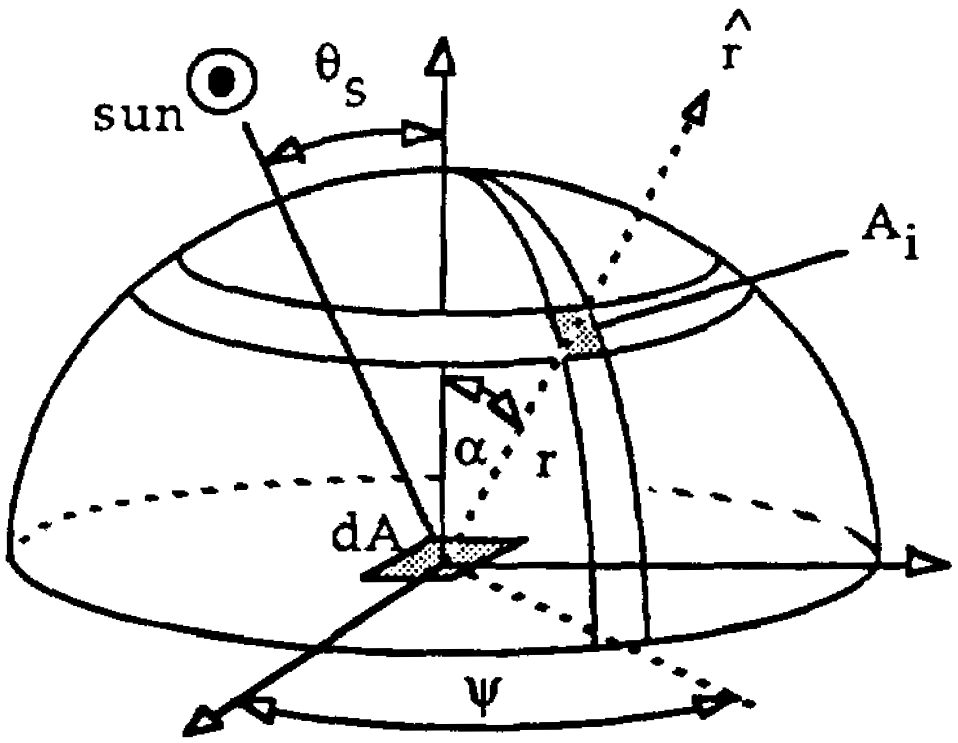
\includegraphics[width=.3\linewidth]{figures/earth_panel_irradiance.png}
   \caption{Geometry of albedo radiation. $dA$ is the source element, $A_i$ is the target.}
   \label{fig:albedo-geometry}
\end{figure}

Albedo radiation, reflected by planet surfaces, is much smaller but still significant. Albedo requires knowledge of properties of the radiation source (for our intents and purposes, the Sun) and the reflecting body. The solar irradiance $E_s$ and angle between reflecting surface normal and Sun $\theta_s$ determine the incident irradiance onto the source surface element $dA$. The reflected radiation depends on the albedo distribution $a=a(\lambda, \phi)$ which may vary with longitude $\lambda$ and latitude $\phi$. The received radiation depends on the view angle $\alpha$, which is the angle between the surface normals of source and target. This geometry is shown in \cref{fig:albedo-geometry}. The reflected radiance depends on the reflectance type. For Earth, purely diffuse Lambertian reflectance is a fair assumption~\cite{Knocke1988}. More sophisticated reflectance considering land cover exist, for example using kernel-based bidirectional reflectance distribution functions (BRDF) as decribed by \textcite{Lucht2000}. The irradiance from $dA$ at the target due to albedo is then given by~\cite{Knocke1988}:
\begin{align}\label{eq:source-albedo-paneled}
   E = a\cos\theta_s E_s\frac{dA\cos\alpha}{\pi \norm{\vb r}^2}
\end{align}
where $a\cos\theta_s E_s$ is the reflected irradiance. Note that albedo radiation only exists if $dA$ receives sunlight. Shadow calculations could also be included but are more involved for albedo models, since both the incoming solar radiation and outgoing albedo radiation could be affected by occultation. Calculations are further complicated since common occultation models assume spherical sources and not flat surface elements.

The simplest choice for the lunar albedo is the average value of $a=0.12$~\cite{Mueller2021}. A more detailed lunar albedo distribution is the 15x15 spherical harmonics model by \textcite{Floberghagen1999}. However, for calculations, paneling of the source is more convenient. \textcite{Knocke1988} introduce a spherical cap centered at the subsatellite point, which is divided into rings of panels of constant albedo, tangent to the source surface at their center. \cref{eq:source-albedo-paneled} is then evaluated for each panel $dA$. We call this \emph{dynamic paneling}. Alternatively, the whole body could be paneled independently of the satellite position (\emph{static paneling}). Such an approach including evenly distributed panels is described by \textcite{Wetterer2014}.

Similarly, the thermal radiation can be described, scaled by the emissivity $e$. Additionally, there is a factor of $1/4$, which is the ratio between receiving and emitting surface. Then the irradiance from $dA$ at the target due to thermal radiation is given by~\cite{Knocke1988}:
\begin{align}\label{eq:source-thermal-knocke}
   E = \frac{e E_s}{4} \frac{dA\cos\alpha}{\pi \norm{\vb r}^2}
\end{align}
where $e E_s/4$ is the emitted exitance. Thermal radiation exists independent of incident sunlight and is therefore constant. The simplest model for lunar emissivity is a constant value of $e=0.95$~\cite{Mueller2021}.

Alternatively, a latitude- and local time-dependent temperature distribution of the lunar surface can be assumed~\cite{Lemoine2013}. By the Stefan--Boltzmann law, the irradiance at the target due to the thermal radiation is given by:
\begin{align}\label{eq:source-thermal-lemoine}
   E = e\sigma T^4 \frac{dA\cos\alpha}{\pi \norm{\vb r}^2}
   \qquad
   T = \max\left(T_\text{max}(\cos\theta_s)^{1/4}, T_\text{min}\right)
\end{align}
where $T_\text{max}=\SI{375}{K}$ and $T_\text{min}=\SI{100}{K}$. Note that the maximum irradiance from \cref{eq:source-thermal-lemoine} is about four times higher than that from \cref{eq:source-thermal-knocke} since $\sigma T_\text{max}^4 \approx E_s$, but the irradiance from \cref{eq:source-thermal-lemoine} varies as the $dA$ moves away from the subsolar point ($\theta_s$ increases) and cools down.

Instead of modeling outgoing planetary fluxes, they can also be observation-based. For Earth, CERES provides time series for shortwave and longwave fluxes with up to hourly and \ang{1} resolution~\cite[]{Doelling2016}. For the Moon, irradiance spectra have been published by \textcite{Kieffer2005} and \textcite{Sun2021}. However, they are constant in time and provide a single spectrum for only the Earth-facing lunar side. Therefore, they are of little use for radiation pressure models in lunar orbits, but can be used for Earth orbits.



\subsection{Targets}
The \emph{cannonball model} is the simplest model for target acceleration due to radiation pressure. The target is modeled as a sphere such that lateral accelerations cancel and there is only an acceleration away from the source along $\vu r$. The cross-sectional area $A$ is independent of orientation, and surface properties (reflectance and absorptivity) are captured in the radiation pressure coefficient $C_r$. Then the acceleration of a target with mass $m$ is given by~\cite{Knocke1988}:
\begin{align}
   \vb a = C_r \frac{A}{m} \frac{E}{c} \vu r
\end{align}

A more sophisticated paneled target model discretizes the spacecraft into $n$ panels with area $A$ and normal vector $\vb n$. This also means that the incidence angle $\theta$ differs per panel. Their surface is characterized by the absorptivity $C_a$, diffuse reflectivity $C_d$ and specular reflectivity $C_s$, which obey $C_a + C_d + C_s = 1$. Anisotropy can be accounted for using BRDFs as described by \textcite{Wetterer2014}. However, we assume Lambertian diffuse reflectance and instantaneous Lambertian reradiation of absorbed radiation.  Then the acceleration of the whole target due to all target panels and a single source is given by~\cite{Montenbruck2014}:
\begin{align}
   \vb a = \frac{1}{m} \frac{E}{c} \sum_{j=1}^n A \cos\theta \left[(C_a + C_d)\left(\vu r - \frac{2}{3} \vb n\right) - 2 C_s \cos\theta \, \vb n \right]
\end{align}
where all quantities inside the summation except $\vu r$ are specific to panel $j$. For the LRO, these panel properties are given by \textcite{Smith2008}. Self-shadowing could also be included here. \textcite{Mazarico2009} describe an algorithm to modify the effective area due to self-shadowing and describe the effect on the spacecraft trajectory as significant. \textcite{Kenneally2020} perform raytracing for self-shadowing with BRDFs on GPUs.

In case of a paneled source, the total acceleration is the vectorial sum of these contributions over all $m$ source panels:
\begin{align}
   \vb a = \frac{1}{m} \sum_{i=1}^m \frac{E}{c} \sum_{j=1}^n A \cos\theta \left[(C_a + C_d)\left(\vu r + \frac{2}{3} \vb n\right) + 2 C_s \cos\theta \, \vb n \right]
\end{align}
where $E$ is the irradiance due to the $i$-th source panel.







\section{Options}
Radiation pressure models range from the simple baseline model to our extended model, but even more configuration options are possible. An extensive overview over options for radiation pressure modeling is given in \cite[Sec.~2]{Vielberg2020}. This list contains all options that have been explored in literature and that Tudat may want to support in the future, hence provisions for extensibility should be made. However, only the \textbf{bold options} will be implemented in this project.

\begin{itemize}
   \item Body:
   \begin{itemize}
      \item \textbf{Mass}
      \item \textbf{Position and orientation}
      \item Shape (for occultation, spherical or oblate spheroid)
      \item Athmosphere (for refraction influencing occultation)
      \item \textbf{Radiation source and/or target}
      \item \textbf{Temperature distribution (in case Lemoine thermal model is used)}
   \end{itemize}
   \item Point source:
   \begin{itemize}
      \item \textbf{Luminosity or TSI (constant or time-varying)}
      \item Continuous or discrete emission spectrum (i.e. function of wavelength, binned or visible + infrared)
   \end{itemize}
   \item Paneled source:
   \begin{itemize}
      \item \textbf{Original radiation source}
      \item \textbf{Albedo and emissivity distribution (constant, per panel or as spherical harmonics)}
      \item \textbf{Thermal emission model (Knocke or Lemoine)}
      \item \textbf{Albedo reflection law (constant} or BRDF, possibly depending on wavelength)
      \item \textbf{Paneling resolution}
      \item \textbf{Static or dynamic paneling}
      \item \textbf{Occultation of albedo panels}
      \item Observation-based fluxes (like CERES measurements) instead of modeled fluxes
   \end{itemize}
   \item Cannonball target:
   \begin{itemize}
      \item \textbf{Cross-sectional area}
      \item \textbf{Radiation pressure coefficient}
   \end{itemize}
   \item Paneled target:
   \begin{itemize}
      \item \textbf{Area of each panel}
      \item \textbf{Position and orientation of each panel (constant} or time-varying (for HGA or SA), from CK kernels or e.g. aligned with sun, position only relevant for self-shadowing and self-reflection)
      \item With or \textbf{without} self-shadowing and self-reflection
      \item \textbf{Absorptivity, specular reflectivity and diffuse reflectivity of each panel (constant} or depending on wavelength, possibly time-varying due to degradation)
      \item \textbf{Reflection law (constant} or BRDF, possibly depending on wavelength)
      \item \textbf{Thermal reradiation (instantaneous} or from temperature distribution considering heat conduction and generation, should be implemented as separate acceleration class if not instantaneous)
   \end{itemize}
\end{itemize}







\section{Verification \& Validation}
Verification will check whether the models presented in this document were implemented correctly, based on manual calculations and values from literature. Validation will check whether the mathematical models themselves give sensible results. Both will be implemented as unit tests. Existing radiation pressure unit tests within Tudat will be reused and adapted to avoid regression. However, existing tests include a lot of logic that itself may be flawed. Therefore, the reworked unit tests will be more straightforward, at the cost of duplicate code.

The lunar radiation model can be rougly validated with the peak lunar irradiance in LRO's lunar orbit of \SI{1330}{W/m^2}~\cite{Tooley2010}. To validate the simulation setup, I will also propagate LRO's orbit and check consistency with ephemerides from SPICE SPKs. While (possibly significant) differences are expected in both, the error should be reasonable and orders of magnitude of results similar.







\section{Result analysis}\label{sec:result-analysis}
The question to be answered is \textit{What is the quantitative influence of using high-accuracy radiation pressure models on the attainable orbit precision for the Lunar Reconaissance Orbiter?} The answer will not include statements about absolute or relative precision improvements, since there is no ground truth. Rather, the answer will give tendencies about how different models and parameters influence orbital elements.

The simulation setup for gathering results will be varied to investigate different levels of accuracy. In the simplest form, the radiation pressure models only contain a direct solar radiation source and a cannonball target without occultation (\emph{baseline model}) In the most complete form (\emph{extended model}), the setup looks as follows:
\begin{itemize}
   \item Sun:
   \begin{itemize}
      \item Ephemeris from DE 421 (used by JPL for LRO ephemeris generation)
      \item Gravity field
      \item Direct solar radiation source
   \end{itemize}
   \item Earth:
   \begin{itemize}
      \item Ephemeris from DE 421
      \item Gravity field
      \item Occulting body for direct solar and lunar albedo radiation
   \end{itemize}
   \item Moon:
   \begin{itemize}
      \item Global origin
      \item Ephemeris from DE 421
      \item Gravity field
      \item Albedo radiation source (paneled Moon with albedo obtained from DLAM-1)
      \item Thermal radiation source (paneled Moon)
      \item Occulting body for direct solar radiation
   \end{itemize}
   \item LRO:
   \begin{itemize}
      \item Propagated (translational) for 565 min, corresponds to about 5 orbital revolutions
      \item Rotational ephemeris
      \item Initial ephemeris from LRO reprocessed spacecraft ephemeris (\texttt{fdf36\_...}) during regular science mission at 50 km altitude, ensure no stationkeeping but eclipses occured during propagation period (start at 26 June 2010 06:00:00)
      \item Paneled radiation pressure target with areas and coefficients from \textcite{Smith2008} (assume SA is pointed towards Sun and HGA is pointer towards Earth)
      \item No self-shadowing, unless time permits
   \end{itemize}
\end{itemize}

The result analysis is inspired by \textcite{Vielberg2020} for LEO satellites, but less involved since a lot of details (e.g. observed outgoing fluxes, observed solar irradiance, land coverage) do not exist for or apply to the Moon. The analysis will consider the following aspects:
\begin{itemize}
   \item Accelerations due to each radiation pressure component (direct solar, albedo, thermal) in radial, cross-track and along-track directions with extended model (cf.~\cite[Fig.~3]{Vielberg2020})
   \item Dependence of accelerations on position in orbit and time (cf.~\cite[Fig.~7]{Vielberg2020}), correlate with relative sun position and albedo map
   \item Sensitivity analysis for albedo and target reflection/absorption coefficients (since these parametrizations are often inaccurate, investigating influence of their errors is important)
   \item Effect of different levels of detail of radiation pressure models on accelerations (cf.~\cite[Fig.~8]{Vielberg2020}) and Keplerian orbit elements (e.g., how does addition of albedo radiation change semi-major axis?), moving from baseline model towards extended model
   \begin{itemize}
      \item Baseline model: only direct solar radiation source, cannonball target, no occultation
      \item For source, add albedo and thermal radiation (vary paneling resolution, constant and spherical harmonics albedo, constant or varying thermal radiation from \cref{eq:source-thermal-knocke,eq:source-thermal-lemoine}, dynamic/static paneling)
      \item For target, switch to paneled model with/without self-shadowing
      \item Add multiple occultation
      \item Compare mean difference and RMS difference w.r.t. baseline in radial, cross-track and along-track directions after propagation arc
      \item Compare Keplerian orbits w.r.t. baseline after propagation arc
      \item Measure performance impact of increased level of detail through wall-clock and/or CPU time, and memory footprint
   \end{itemize}
\end{itemize}







\section{Code design}
All models presented in \cref{sec:models} will be implemented. The following Python-like pseudocode shows the classes and their interactions. The code is not complete but only contains parts relevant for radiation pressure computations.

All radiation source and target calculations are performed in their respective local frames. The \pythoninline{class RadiationPressureAcceleration} handles reference frame transformations between them. This simplifies and decouples source and target code.

\inputminted{python}{code_design.py}







\section{Implementation plan}
A minimum viable version will be implemented first, including only a point source and a cannonball target (the baseline model). Once this version works and has been verified, the more complex models can follow. All implementations also include unit tests for verification and validation. The implementation plan is as follows:
\begin{enumerate}
   \item Implement baseline model
   \begin{enumerate}
      \item Implement \pythoninline{class IsotropicPointRadiationSourceModel} with abstract base class
      \item Implement \pythoninline{class CannonballRadiationPressureTargetModel} with abstract base class
      \item Implement \pythoninline{class RadiationPressureAcceleration} without occultation
      \item Implement LRO simulation (baseline model)
      \item Verify functionality and check if design makes sense
   \end{enumerate}
   \item Implement \pythoninline{class PaneledRadiationPressureTargetModel} 
   \item Implement \pythoninline{class PaneledRadiationSourceModel} with static paneling (constant albedo until we get access to DLAM-1)
   \item Implement \pythoninline{class OccultationGeometry} for single occulting body and include in \\ \pythoninline{class RadiationPressureAcceleration}
   \item Implement LRO simulation (extended model) as described in \cref{sec:result-analysis}
   \item Validate complete simulation
   \item Implement extra items, if time permits
   \begin{enumerate}
      \item Implement spherical harmonics lunar albedo model DLAM-1 from \textcite{Floberghagen1999}, if we get access
      \item Implement occultation by two bodies from \textcite{Zhang2019}
      \item Implement \pythoninline{class PaneledRadiationSourceModel} with dynamic paneling
      \item Implement self-shadowing from \textcite{Mazarico2009}
      \item Optimize
   \end{enumerate}
\end{enumerate}







\printbibliography

\end{document}
